
\documentclass[10pt, openany]{book}

%PACKAGES%

\usepackage[inner=0.75in, outer=0.75in, top=0.75in, bottom=0.75in, a5paper]{geometry}
\usepackage{graphicx}
\usepackage{fontspec, newunicodechar}
%\usepackage{sectsty}
\usepackage{titlesec}
\usepackage{verse}
\usepackage[unicode, pdfauthor={Bhikkhu Sunyo}, pdftitle={Viññāṇa Anidassana: The state of boundless consciousness}, pdfsubject={Buddhism}, pdfkeywords={Buddhism}, pdfcreator={Wiswo-texBuilder}, hyperfootnotes=false]{hyperref} 

%links and cites
\hypersetup{
    colorlinks = true,
    linkcolor = [rgb]{0.1, 0.1, 0.56},
    anchorcolor = blue,
    citecolor = blue,
    filecolor = blue,
    urlcolor = [rgb]{0.4, 0.6, 0.91}
    }

%MICROTYPOGRAPHY%
\usepackage{microtype}

\hyphenpenalty=750

%LINESPACE%
\usepackage{setspace}
\setstretch{1.20}
\setlength{\parskip}{0pt}

%Minimum space before footnotes
\setlength{\skip\footins}{1\baselineskip}
\setlength{\footnotesep}{11pt}

%VERSE%
\settowidth{\versewidth}
{mmmmmmmmmmmmmmmmmmm}%THIS SETS THE GLOBAL DEFAULT WIDTH OF CENTERING. IT IS USUALLY DETERMINED LOCALLY, HOWEVER.%
%VERSE%


%HEADER%
\usepackage{fancyhdr}
\setlength{\headheight}{15pt}
\pagestyle{fancy}

\fancyhf{}
%\fancyfoot[CE,CO]{– \thepage \hspace{0.18em}–}

\fancyhead[RO]{\headerfont\scshape\small\textcolor[rgb]{0.5, 0.5, 0.5}{Viññāṇa Anidassana —\hspace{0.18em}\thepage}}
\fancyhead[LE]{\headerfont\scshape\small\textcolor[rgb]{0.5, 0.5, 0.5}{\thepage\hspace{0.18em}— Bhikkhu Sunyo}}

\renewcommand{\headrulewidth}{0pt}
\fancypagestyle{plain}{ %
\fancyhf{} % remove everything
\renewcommand{\headrulewidth}{0pt}
\renewcommand{\footrulewidth}{0pt}
}

\renewcommand\footnoterule{{\color[rgb]{0.8, 0.8, 0.8} \hrule width 1in height 0.2pt}} % a 1 inch gray line 


%FONTS%
\setmainfont[]{Gentium Book Plus}
\setsansfont[]{Linux Biolinum O}
%FONTS%

\titleformat{\chapter}
{\center\Huge\Chapfont\scshape}
{}
{0pt}
{}

\titleformat{\section}
{\linespread{0.75}\center\Large\scshape\Secfont}
{}
{0pt}
{}

\setcounter{secnumdepth}{-1}

\newfontfamily\Chapfont[]{Wiswo Small Caps}
%\newfontfamily\Chapnumfont{Source Sans 3}
\newfontfamily\Secfont[]{Wiswo Small Caps}
%\sectionfont{\linespread{0.75}\center\Large\Secfont}
\newfontfamily\headerfont[]{Wiswo Small Caps}

\newfontfamily\Titlefont[]{Wiswo Small Caps}

%EPIGRAPH%
\newenvironment{epigraph}


%HANGING LEFT%
\newcommand*{\vleftofline}[1]{\leavevmode\llap{#1}}

%WIDOWS & ORPHANS%
\widowpenalty=10000
\clubpenalty=10000

\counterwithout{footnote}{chapter}
\usepackage[hang,flushmargin,bottom]{footmisc}
%\graphicspath{ {./images/} }

\newcommand{\nocontentsline}[3]{}
\newcommand{\tocless}[2]{\bgroup\let\addcontentsline=\nocontentsline#1{#2}\egroup}

\makeatletter
\newcommand{\epubchapter}[1]{%
  \begingroup
  \let\@makechapterhead\@gobble % make \@makechapterhead do nothing
  \tocless \chapter{#1}
  \endgroup
}
\makeatother

\usepackage{verbatim}


\pretolerance=400
\tolerance=800
\emergencystretch=3pt

\newenvironment{aphorism}%
{%
\begin{center}\begin{itshape}
}%
{\end{itshape}\end{center}
}%

\hyphenation{manu-scripts}


\begin{document}

\frontmatter

\pagestyle{empty}

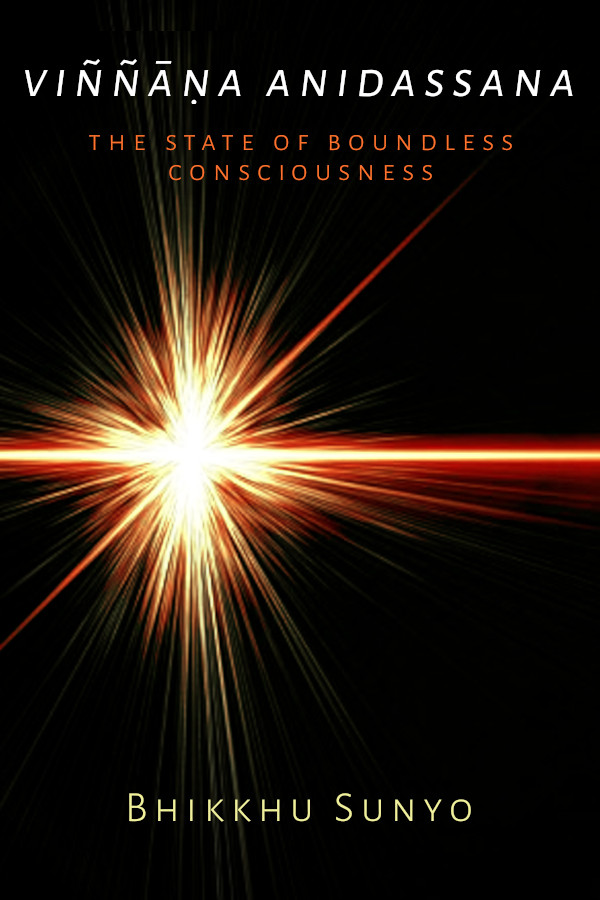
\includegraphics[scale= 2, trim= 0 0 0 0]{../_resources/book-data/vasy/FrontLarge.jpg}

\newpage~\newpage~

\begin{center}
\vspace{2em}

\Huge\Titlefont\scshape{Viññāṇa Anidassana}\\
\vspace{0.5em}
\large\Titlefont\scshape{The state of boundless consciousness}\\

\begin{Large}
\vspace{4em}
\Titlefontscshape{Bhikkhu Sunyo}
\end{Large}


\vspace*{\fill}

\includegraphics[scale=0.06, trim = 0 13 5 0 ]{../_resources/images/icons/logo-enso-large}\\
\vspace{4pt}
\begin{small}
\scshape{Wisdom \& Wonders\\
Books}
\end{small}
\end{center}

\newpage
\begin{small}
\begin{sffamily}
\noindent Copyright © — Bhikkhu Sunyo\\

\noindent Originally published in 2021.\\\noindent This edition published in 2022.\\\noindent Addendum added 2024.\\

\noindent\textbf{CC0 1.0 Universal (CC0 1.0) Public Domain Dedication}\\



\noindent\textbf{No Copyright}

\noindent The person who associated a work with this deed has dedicated the work to the public domain by waiving all of his or her rights to the work worldwide under copyright law, including all related and neighboring rights, to the extent allowed by law.

\noindent You can copy, modify, distribute and perform the work, even for commercial purposes, all without asking permission. See Other Information below.


\noindent\textbf{Other Information}

\noindent In no way are the patent or trademark rights of any person affected by CC0, nor are the rights that other persons may have in the work or in how the work is used, such as publicity or privacy rights.

\noindent Unless expressly stated otherwise, the person who associated a work with this deed makes no warranties about the work, and disclaims liability for all uses of the work, to the fullest extent permitted by applicable law.

\noindent When using or citing the work, you should not imply endorsement by the author or the affirmer.

\end{sffamily}
\end{small}

\end{document}